\documentclass{article}
\usepackage{color}
\usepackage[margin=1in]{geometry}
\usepackage[utf8]{inputenc}
\usepackage{amsmath,amsfonts,amssymb}
\usepackage{graphicx}
\usepackage{tikz}
\usetikzlibrary{automata,positioning}

% convenience macro
\newcommand{\mat}[1]{\begin{bmatrix}#1\end{bmatrix}}
\newcommand{\vect}[1]{\begin{bmatrix}#1\end{bmatrix}}

\title{PS10}
\author{Giacomo Cappelletto}
\date{}

\begin{document}
\maketitle

\section*{1}

\subsection*{A}
We require each row of $A$ to sum to 1:
\[
\begin{cases}
0.6 + 0.2 + \alpha = 1,\\
0.2 + \beta + 0.2 = 1,\\
\gamma + 0.2 + 0.6 = 1.
\end{cases}
\quad\Longrightarrow\quad
\alpha=0.2,\ \beta=0.6,\ \gamma=0.2,
\]
hence
\[
A=\mat{
0.6 & 0.2 & 0.2\\
0.2 & 0.6 & 0.2\\
0.2 & 0.2 & 0.6
}.
\]

\subsection*{B}
Write $A=(a_{ij})$ and draw its transition diagram:
\begin{center}
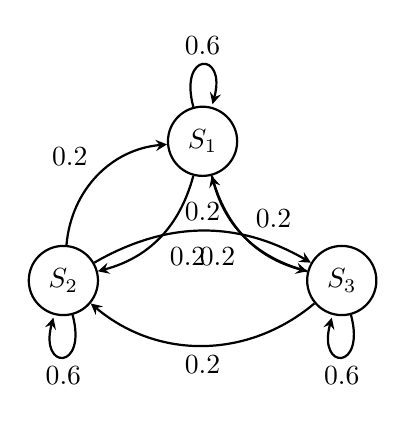
\begin{tikzpicture}[->,>=stealth,auto,node distance=2.5cm, thick]
  \node[state] (S1)               {$S_1$};
  \node[state] (S2) [below left of=S1]   {$S_2$};
  \node[state] (S3) [below right of=S1]  {$S_3$};
  \path
    (S1) edge[loop above]    node{0.6} (S1)
         edge[bend left]     node{0.2} (S2)
         edge[bend right]    node{0.2} (S3)
    (S2) edge[loop below]    node{0.6} (S2)
         edge[bend left]     node{0.2} (S3)
         edge[bend left=40]  node{0.2} (S1)
    (S3) edge[loop below]    node{0.6} (S3)
         edge[bend left]     node{0.2} (S1)
         edge[bend left=40]  node{0.2} (S2);
\end{tikzpicture}
\end{center}

\subsection*{C}
From (A): $\alpha=0.2,\ \beta=0.6,\ \gamma=0.2$.

\subsection*{D}
Compute the characteristic polynomial:
\[
\det(A-\lambda I)
=\det\mat{
0.6-\lambda & 0.2 & 0.2\\
0.2 & 0.6-\lambda & 0.2\\
0.2 & 0.2 & 0.6-\lambda
}
\]
\begin{align*}
&=(0.6-\lambda)\bigl[(0.6-\lambda)^2-0.04\bigr]
-0.2\bigl[0.2(0.6-\lambda)-0.04\bigr]
+0.2\bigl[0.04-0.2(0.6-\lambda)\bigr]\\
&=(0.6-\lambda)(\lambda^2-1.2\lambda+0.32)
-0.2(-0.12+0.2\lambda)
+0.2(0.04-0.2\cdot0.6+0.2\lambda)\\
&=(0.6-\lambda)(\lambda^2-1.2\lambda+0.32)
+0.024-0.04\lambda
+0.008-0.04\lambda\\
&=-\lambda^3+1.8\lambda^2-0.96\lambda+0.16\\
&=-(\lambda-1)(\lambda^2+0.8\lambda-0.16).
\end{align*}

\subsection*{E}
Solve the quadratic factor:
\[
\lambda^2+0.8\lambda-0.16=0
\quad\Longrightarrow\quad
-\bigl(\lambda^2-0.8\lambda+0.16\bigr)=0
\quad\Longrightarrow\quad
(\lambda-0.4)^2=0,
\]
so
\[
\lambda_1=1,\quad \lambda_2=\lambda_3=0.4.
\]

\subsection*{F}
Since $A^T=A$, $A$ is symmetric and thus orthogonally diagonalizable.

\subsection*{G}
If $A=PDP^{-1}$ then
\[
  D^k=\begin{bmatrix}
    \lambda_1^k & 0 & 0\\
    0& \lambda_2^k & 0\\
    0& 0 & \lambda_3^k
    \end{bmatrix}
\]

\subsection*{H}
As $k\to\infty$,
\[
1^k\to1,\qquad 0.4^k\to0.
\]

\subsection*{I}
Find the stationary distribution by solving $(A-I)x=0$:
\[
A-I=\mat{
-0.4 & 0.2 & 0.2\\
0.2  & -0.4& 0.2\\
0.2  & 0.2 & -0.4
}
\ \xrightarrow{\text{row‐reduce}}\ 
\mat{
1 & 1 & 1\\
0 & 0 & 0\\
0 & 0 & 0
}
\quad\Longrightarrow\quad
x_1=x_2=x_3.
\]
Normalized,
\[
\pi=\frac1{3}\vect{1\\1\\1}.
\]

\end{document}
